\documentclass[a4paper,12pt]{article}

\setlength{\textwidth}{15.0cm}
\setlength{\textheight}{24.0cm}
\setlength{\topmargin}{0cm}
\setlength{\headsep}{0cm}
\setlength{\headheight}{0cm}
\pagestyle{plain}

\usepackage{hyperref}
\hypersetup{
    colorlinks=true,
    linkcolor=blue,
    filecolor=magenta,      
    urlcolor=blue,
    citecolor=blue,
    linktoc=page
}
\usepackage[dvips]{epsfig}
\usepackage{tikz}
\usepackage[english]{babel}
\usepackage{caption}
\captionsetup{font=it}
\usepackage[autostyle, english=american]{csquotes}

\usepackage[
backend=biber,
style=alphabetic,
]{biblatex}

\renewcommand{\bibfont}{\footnotesize}

\usepackage{amsmath,amssymb,amsthm}

\usepackage{comment}
\usepackage{listings}

% \addbibresource{bibliography2.bib} 
\setlength{\parindent}{0pt}

\selectlanguage{english}
\begin{document}

\title{Project 2023-2024: Simulation of the Double Slit Experiment
    and simulation of Wi-Fi signals at home}
\author{Isidoor Pinillo Esquivel}
\date{\today}
\maketitle


\section{Exterior Complex Scaling (ECS) boundary conditions}
\subsection{Equivalence of complex grid and complex wave number}

For homogenous the discretized Helmholtz equation ECS is equivalent to
complex wave number. Let $h$ be normal "real" grid spacing and $\tilde{h} = z h, z \in \mathbb{C} $
be the complex grid spacing.
Let $\sigma$ be normal real wave number and $\tilde{\sigma} = z^{2} \sigma$ be the complex wave number.
Let $u$ be the solution to the discretized Helmholtz equation with complex wave number on a normal grid
and $\tilde{u}$ be the solution to the discretized Helmholtz equation on the complex grid.

\begin{align}
    \frac{\tilde{u}(\tilde{x}-\tilde{h}) -2 \tilde{u}(\tilde{x}) + \tilde{u}(\tilde{x} - \tilde{h})}{\tilde{h}^2} + \sigma \tilde{u} & = 0  \Leftrightarrow \\
    \frac{\tilde{u}(\tilde{x}-zh) -2 \tilde{u}(\tilde{x}) + \tilde{u}(\tilde{x} - zh)}{z^{2}h^2} + \sigma \tilde{u}                  & = 0  \Leftrightarrow \\
    \frac{u(x-h) -2 u(x) + u(x - h)}{h^2} + z^{2} \sigma u                                                                           & = 0  \Leftrightarrow \\
    \frac{u(x-h) -2 u(x) + u(x - h)}{h^2} + \tilde{\sigma} u                                                                         & = 0
\end{align}

This equivalence doesn't hold when there is a source term.

\subsection{ non uniform helmhotz matrix}
Our implementation of the non-uniform of the helmholtz equation uses at its base:
$$
    (\Delta_{h}u)_{i} = -\left( \frac{u_{i+1} - u_{i}}{h_{i+1/2}} - \frac{u_{i} - u_{i-1}}{h_{i-1/2}} \right) \frac{2}{h_{i+1/2} +h_{i-1/2}}
    .
$$

\subsection{interpolation matrix}

The interpolation matrix is based on linear interpolation on a irregular grid, we only use
the real part of the complex grid to do interpolation. The restriction operation is defined
through the variational property.

\subsection{Test Problem}

We test our implementation of the vcycle on a point source problem with $\sigma = -10$.

\begin{figure}[h!]
    \centering
    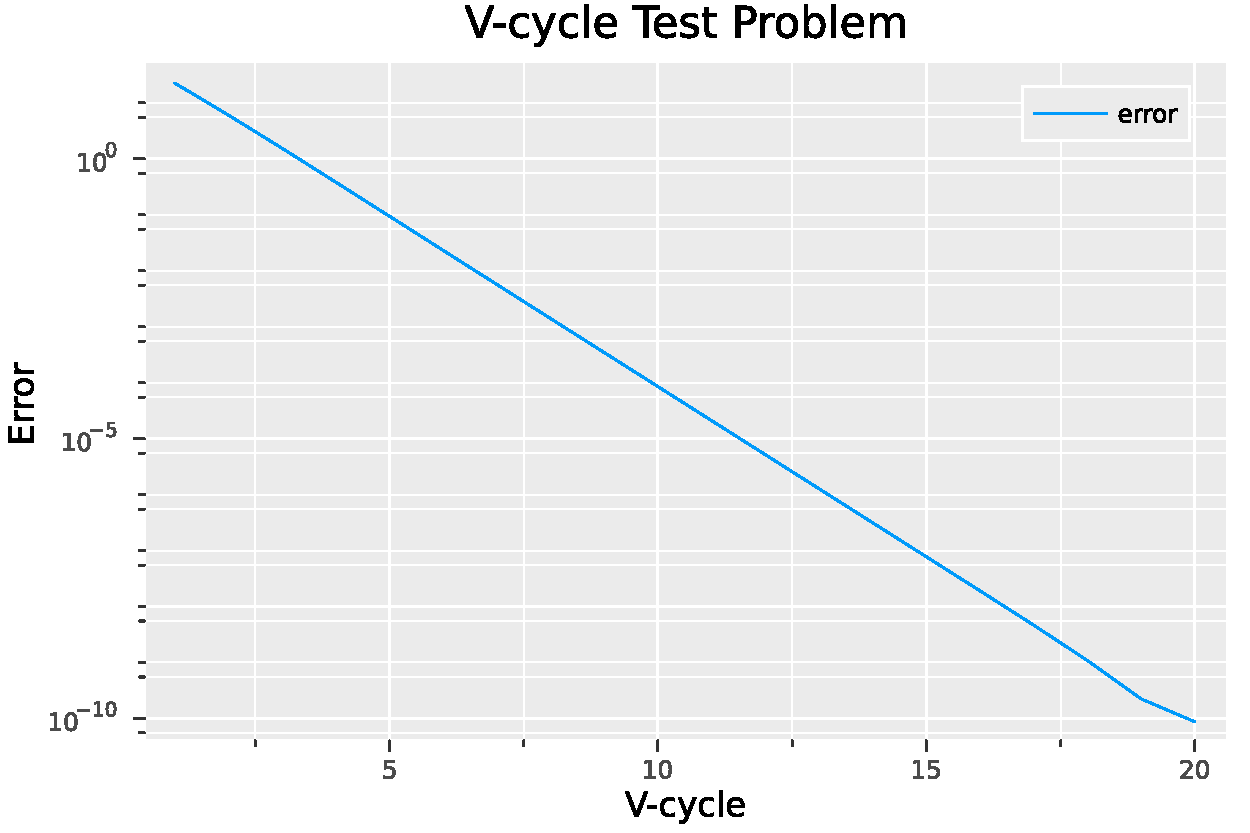
\includegraphics[width=0.8\textwidth]{../plots/Vcycle_Test_Problem.pdf}
    \caption{Convergence of the Vcycle for the test problem.}
    \label{fig:../plots/Vcycle_Test_Problem.pdf}
\end{figure}

\begin{figure}[h!]
    \centering
    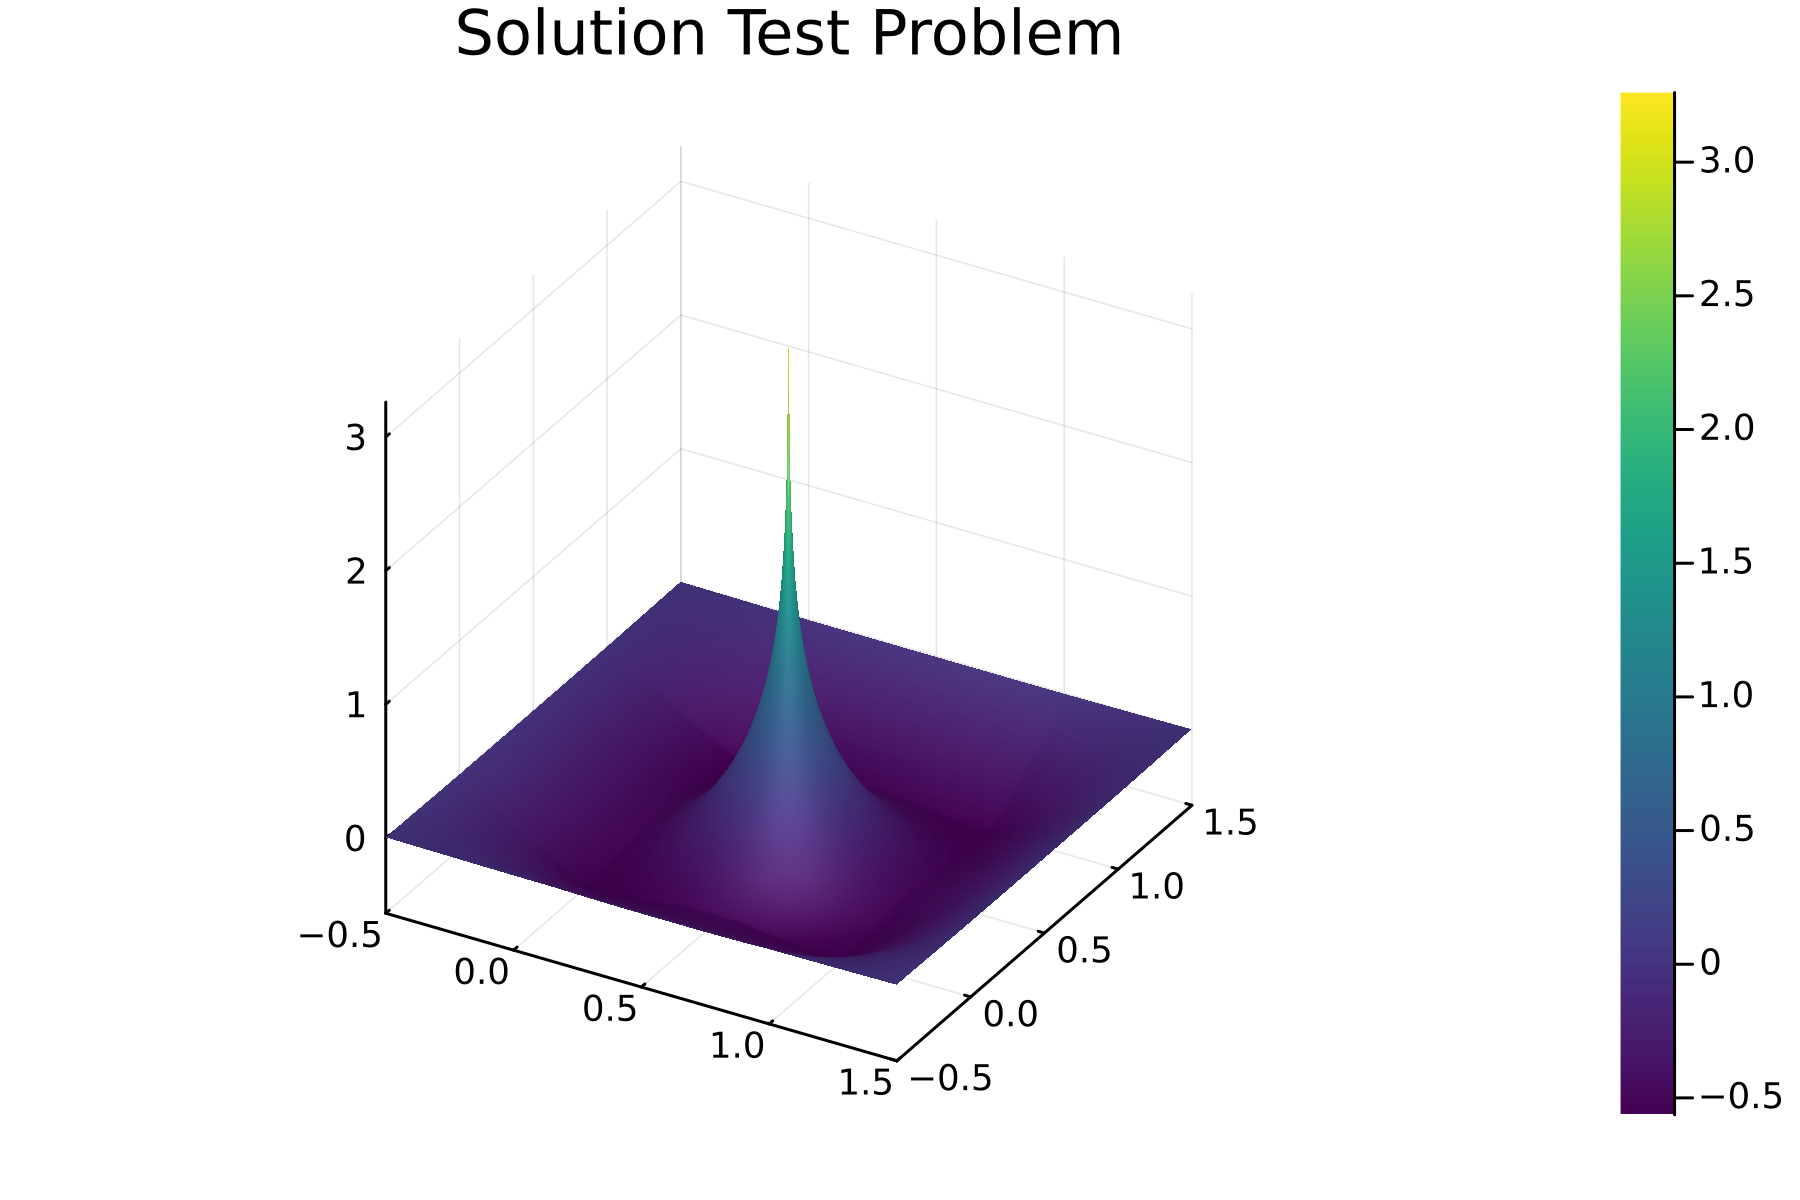
\includegraphics[width=0.8\textwidth]{../plots/Solution_Test_Problem.pdf}
    \caption{Computed solution for the test problem.}
    \label{fig:Solution_Test_Problem}
\end{figure}

\section{Double Slit Experiment}
\subsection{divergence of multigrid 2 slit}

In previous project we studied divergence of the helmholtz equation with homogeneous wavenumber.
Making the wavenumber inhomogeneous doesn't change the divergence of the multigrid method.

\begin{figure}[h!]
    \centering
    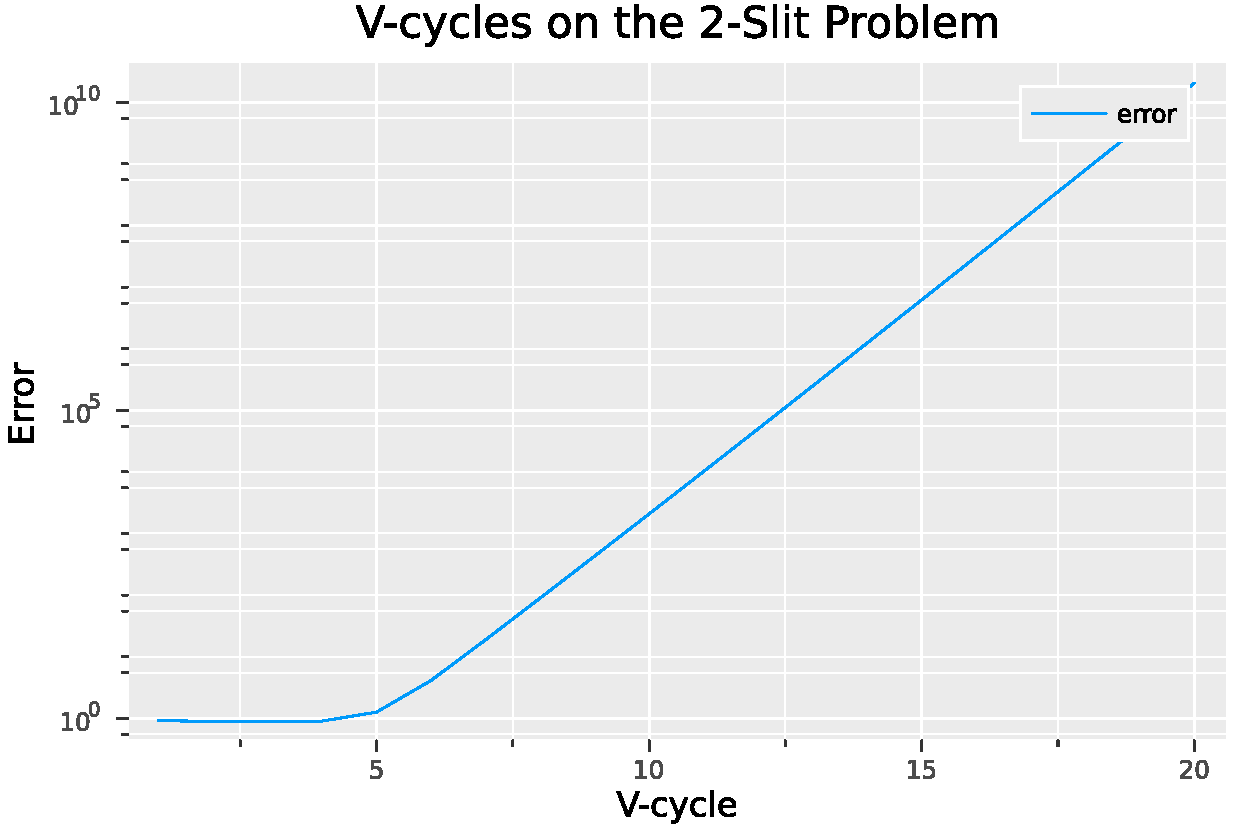
\includegraphics[width=0.8\textwidth]{../plots/Convergence_of_V-cycles_on_the_2-Slit_Problem.pdf}
    \caption{convergence vcycles}
    \label{fig:../plots/Convergence_of_V-cycles_on_the_2-Slit_Problem.pdf}
\end{figure}

\subsection{analysis of ECS Poisson Operator}
Adding ECS to the Poisson operator  make some eigenvalues complex but this doen't explain divergent behavior
of multigrid. What would explain the divergence are the spectral properties of the Helmholtz operator.

\subsection{convergence of shifted multigrid 2 slit}
As in project 1 adding a complex shift helps multigrid converge.
\begin{figure}[h!]
    \centering
    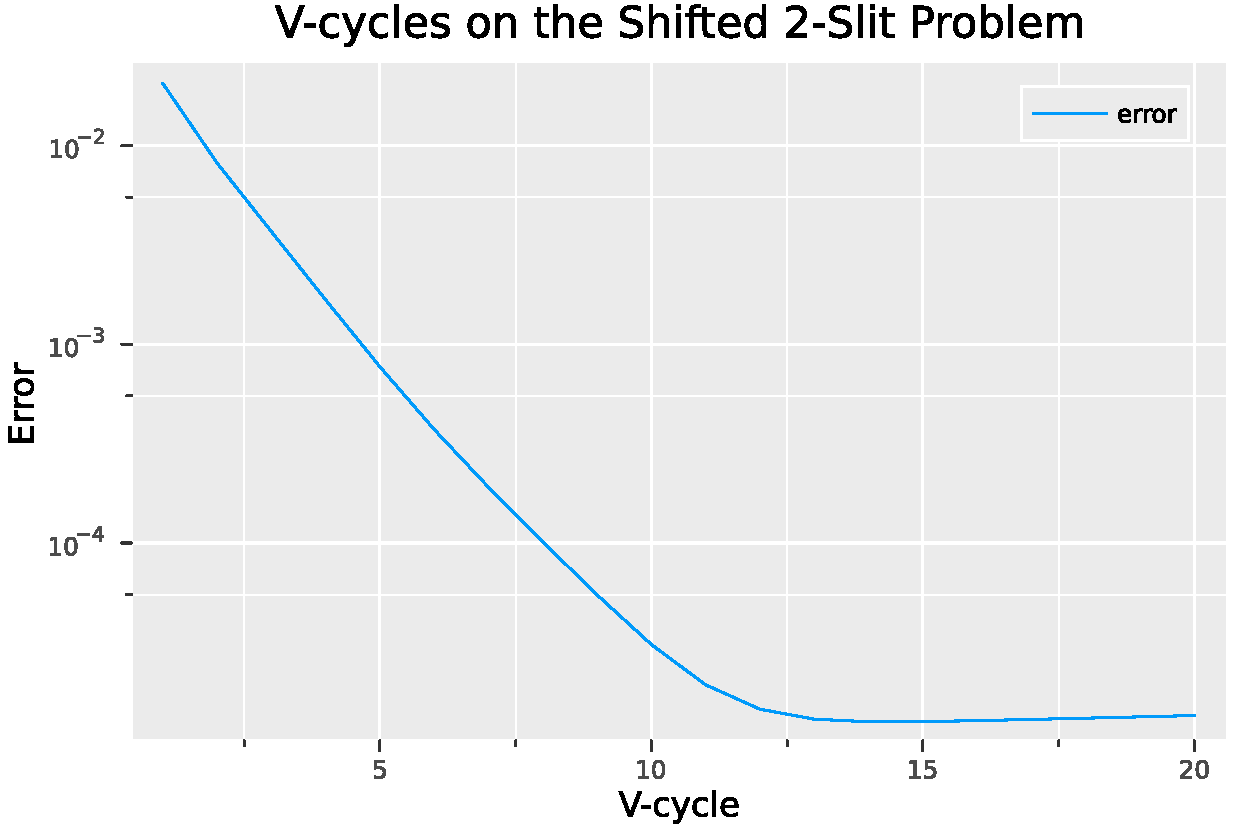
\includegraphics[width=0.8\textwidth]{../plots/Vcycles_shifted2slit.pdf}
    \caption{convergence vcycles shifted}
    \label{fig:../plots/Vcycles_shifted2slit.pdf}
\end{figure}

\subsection{preconditioned GMRES}
The shifted problem can be used as a preconditioner to the non-shifted problem.
\begin{figure}[h!]
    \centering
    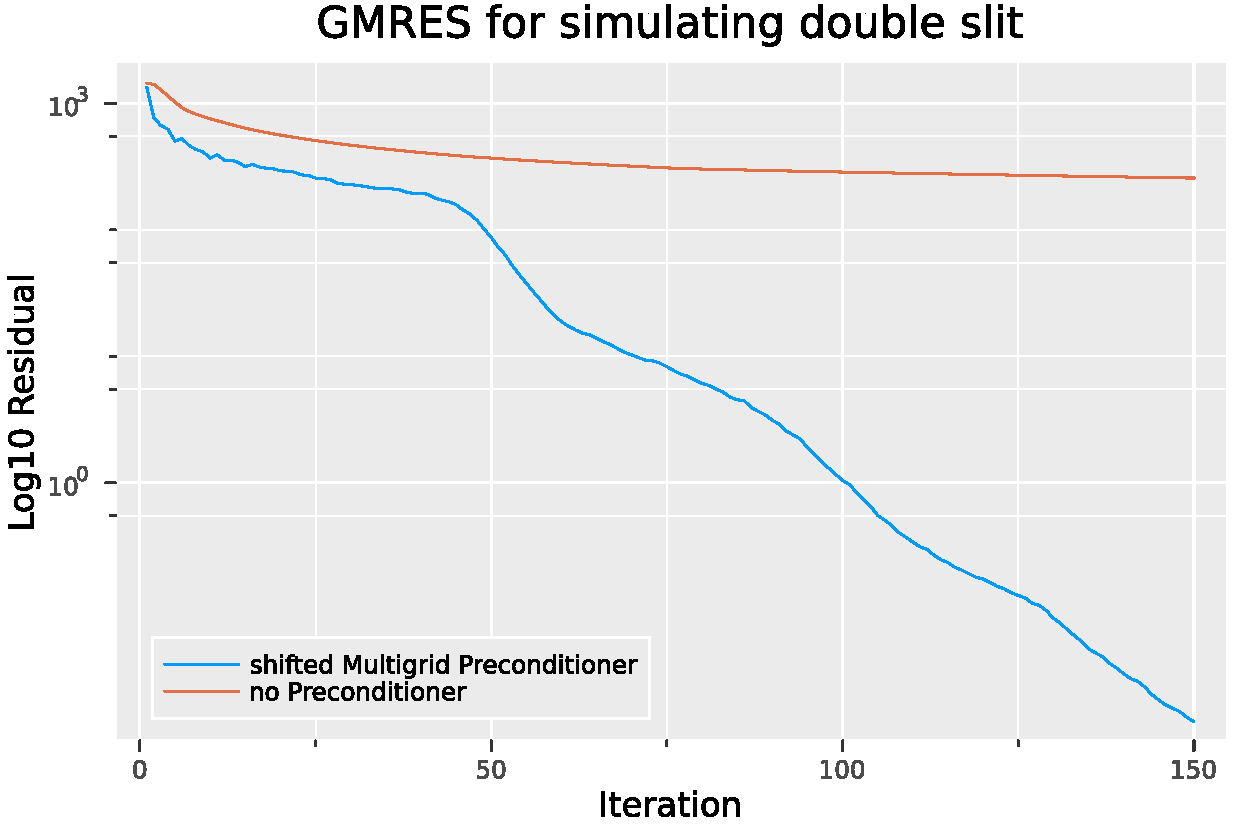
\includegraphics[width=0.8\textwidth]{../plots/GMRES2slit.pdf}
    \caption{convergence preconditioned GMRES}
    \label{fig:../plots/GMRES2slit.pdf}
\end{figure}

\section{Wi-Fi signals at home}

\subsection{wavenumber and source}
We used github copilot to construct the wavenumber and the source representing the house.

\begin{figure}[h!]
    \centering
    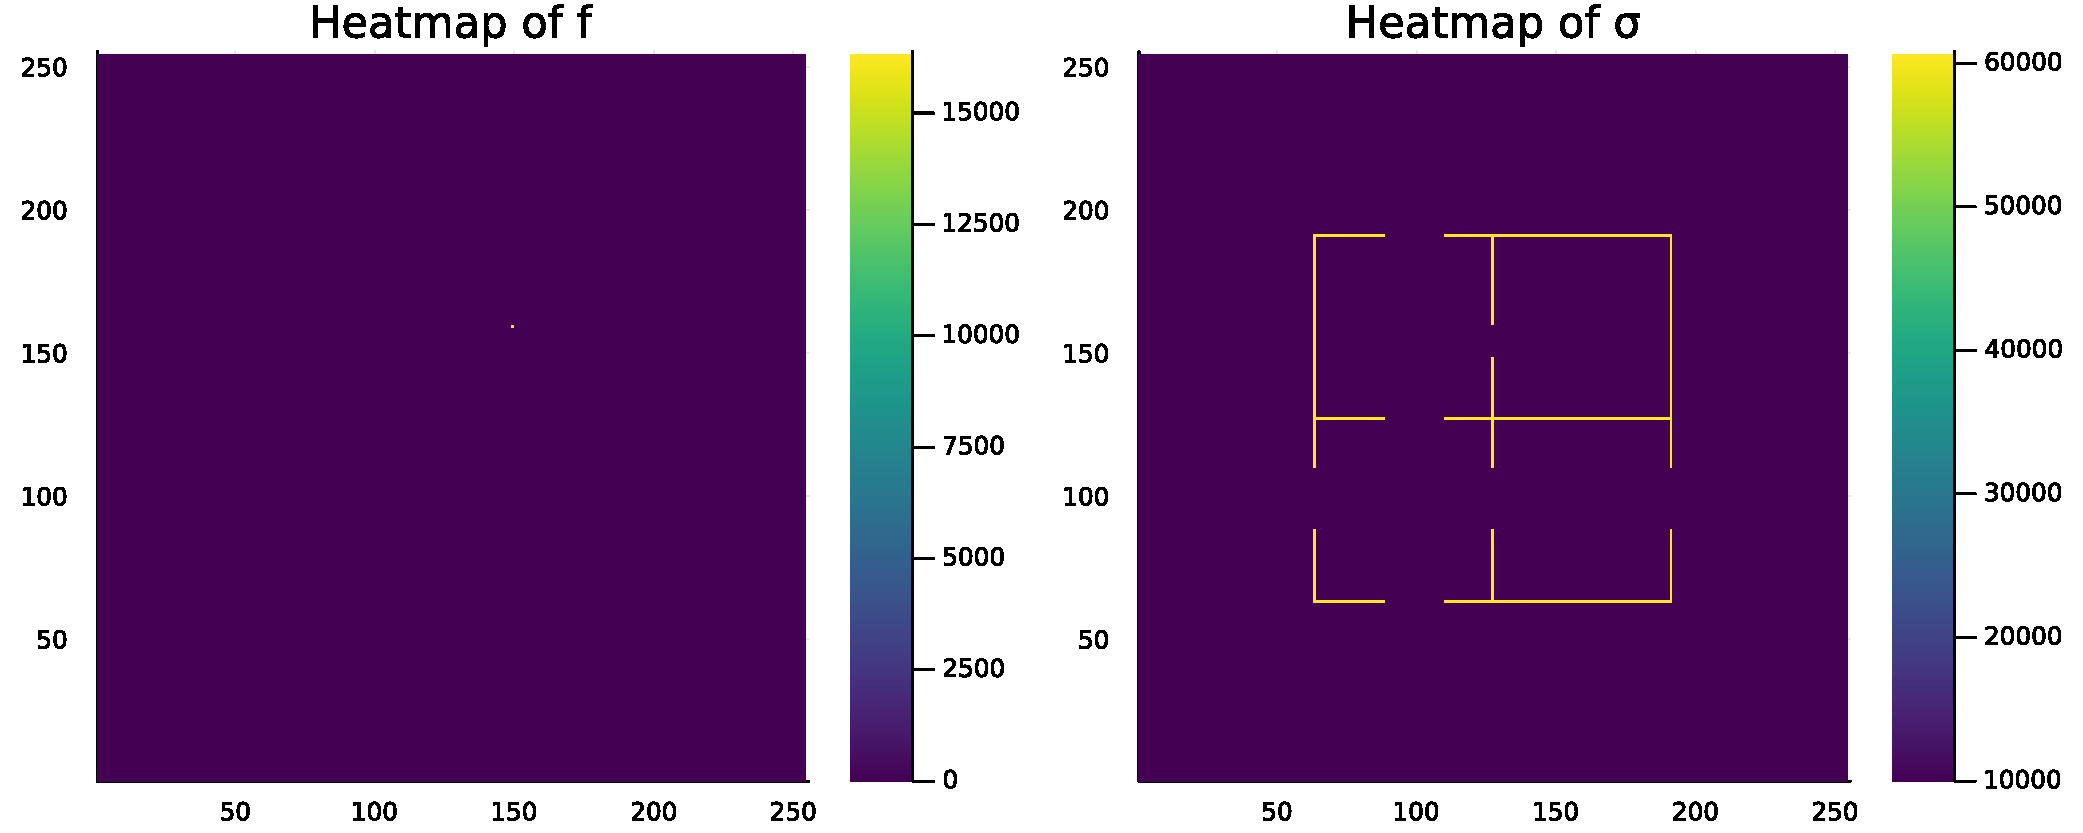
\includegraphics[width=0.8\textwidth]{../plots/wifi_setup.pdf}
    \caption{setup for wifi problem}
    \label{fig:../plots/wifi_setup.pdf}
\end{figure}

\subsection{preconditioned gmres}
This is analogous to the 2 slit problem, we use the shifted problem as a preconditioner to the non-shifted problem.
GMRES takes longer to converge because of worse behaving wavenumber.

\begin{figure}[h!]
    \centering
    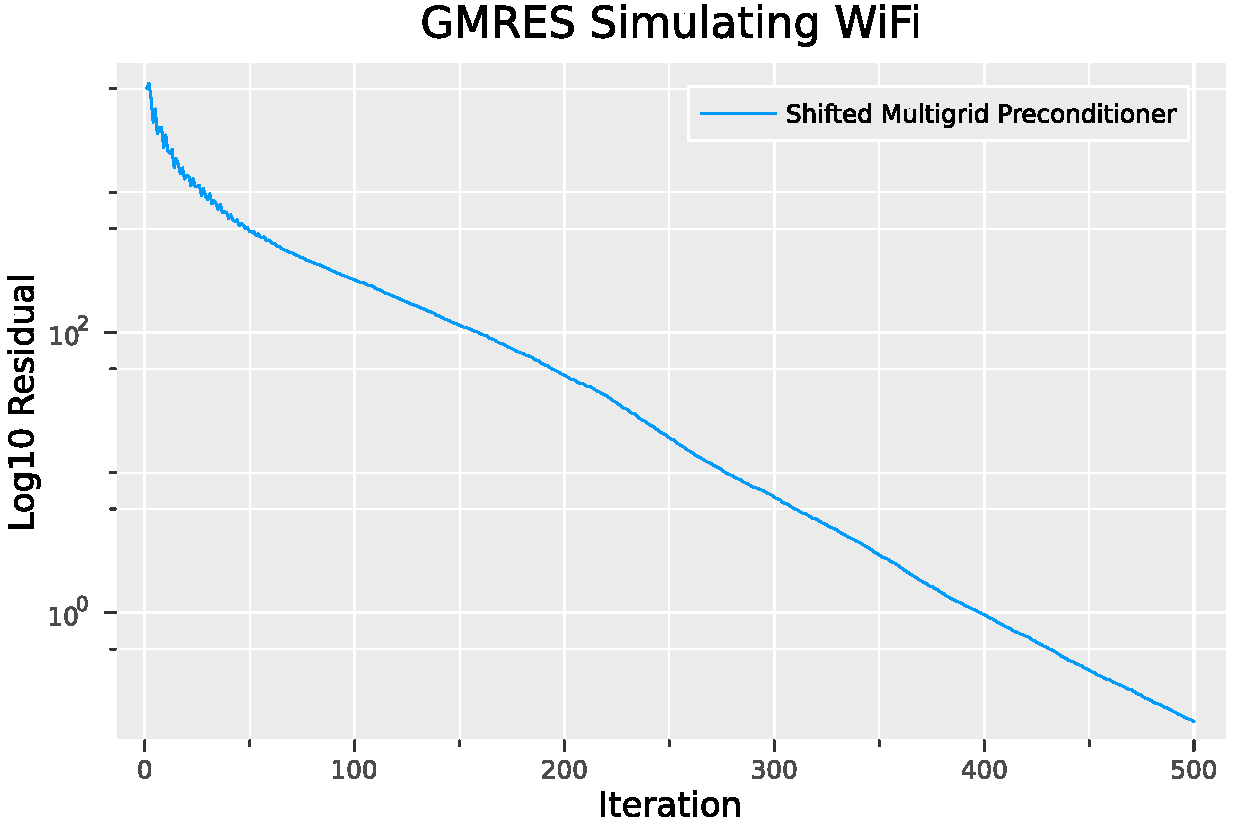
\includegraphics[width=0.8\textwidth]{../plots/gmres_wifi.pdf}
    \caption{convergence plot}
    \label{fig:../plots/gmres_wifi.pdf}
\end{figure}

Here we plot the computed solution to the wifi problem.

\begin{figure}[h!]
    \centering
    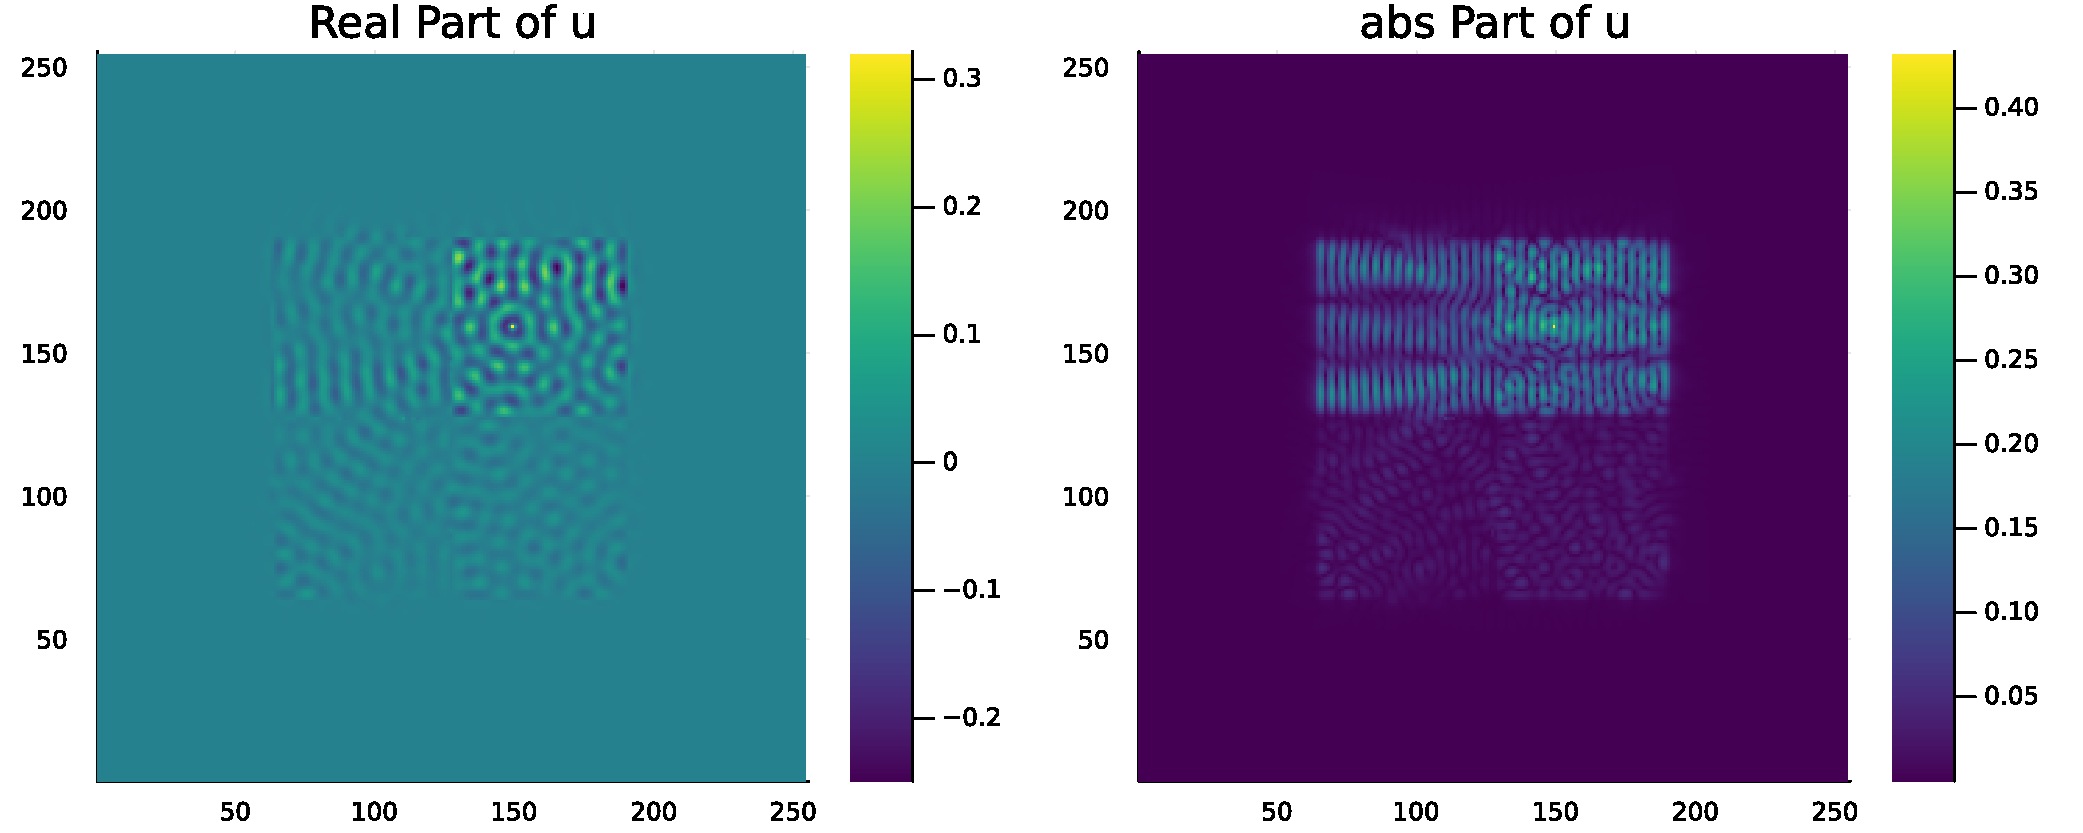
\includegraphics[width=0.8\textwidth]{../plots/gmres_wifi_solution.pdf}
    \caption{solution wifi}
    \label{fig:../plots/gmres_wifi_solution.pdf}
\end{figure}


\end{document}
